%! TEX root = ../../main.tex

\documentclass[main]{subfiles}

\begin{document}

\chapter{図をつくる}

\section{Draw.io}
Draw.ioは,ブラウザ上で動作する図作成ツールである.

\subsection{Draw.ioの埋め込み}
Draw.ioをPDFに変換して,\mintinline{latex}{\includegraphics}で埋め込む.
\path{*.drawio}は,\path{tex/sections/*/fig/drawio/}に保存すると,
\path{tex/sections/*/fig/gen/}にPDFが生成されるので,
PDFのパスを\mintinline{latex}{\includegraphics}で指定する.

\subsection{Draw.ioの埋め込み例}
\subsubsection{ファイルの配置}
\path{tex/sections/figures/fig/drawio/}に\path{figsample.drawio}を配置する(Fig.\ref{fig:drawiofile}).

\begin{figure}[H]
  \centering
  \includegraphics{fig/addfile.png}
  \caption{drawioファイル配置}
  \label{fig:drawiofile}
\end{figure}

\subsubsection{図の編集}

VSCodeエディタの拡張機能で編集する.
ブラウザ上のでも編集できるが,VSCodeの方が便利.

\begin{figure}[H]
  \centering
  \includegraphics[width=0.8\linewidth]{fig/edit.png}
  \caption{drawio編集}
  \label{fig:drawio}
\end{figure}

\subsubsection{図の埋め込み}

\mintinline{latex}{\includegraphics}で図を埋め込む.

\begin{minted}[frame=lines]{latex}
  \begin{figure}
    \centering
    \includegraphics[width=0.8\linewidth]{fig/gen/figsample.pdf}
    \caption{drawio埋め込み}
    \label{fig:drawioinclude}
  \end{figure}
\end{minted}

\begin{figure}[H]
  \centering
  \includegraphics[width=0.8\linewidth]{fig/gen/figsample.pdf}
  \caption{drawio埋め込み}
  \label{fig:drawioinclude}
\end{figure}

\LaTeX{}ファイルをコンパイルすると,PDFが出力されて,図をうめこむことができる.

うまく行かない場合は,中間生成物ディレクトリ\path{tex/out}を消すと良い.

\section{Graphviz(dot)}
Graphviz(dot)は,dot言語で記述したダイアグラムを作成するツールである.

\subsection{Graphviz(dot)の埋め込み}
dotファイルをPDFに変換して,\mintinline{latex}{\includegraphics}で埋め込む.
\path{*.dot}は,\path{tex/sections/*/fig/dot/}に保存すると,
\path{tex/sections/*/fig/gen/}にPDFが生成されるので,
PDFのパスを\mintinline{latex}{\includegraphics}で指定する.

\subsection{Graphviz(dot)の埋め込み例}
\path{tex/sections/figures/fig/dot/}に\path{graph.dot}を配置する.

\begin{minted}[linenos,frame=lines]{dot}
  digraph G {
      rankdir=LR;
      a -> b;
      b -> c;
      c -> d;
      d -> a;
      学生 -> ラーメン [label="吸収"];
      ラーメン -> 学生 [label="健康"];
    }
\end{minted}

\mintinline{latex}{\includegraphics}で図を埋め込む.

\begin{minted}[frame=lines]{latex}
  \begin{figure}
    \centering
    \includegraphics[width=0.8\linewidth]{fig/gen/graph.pdf}
    \caption{dot埋め込み}
    \label{fig:dotinclude}
  \end{figure}
\end{minted}

\begin{figure}[H]
  \centering
  \includegraphics[width=0.8\linewidth]{fig/gen/graph.pdf}
  \caption{dot埋め込み}
  \label{fig:dotinclude}
\end{figure}

\section{PlantUML}
PlantUMLは,PlantUML言語で記述したダイアグラムを作成するツールである.

\subsection{PlantUMLの埋め込み}
PlantUMLファイルをPDFに変換して,\mintinline{latex}{\includegraphics}で埋め込む.

\path{*.pu}は,\path{tex/sections/*/fig/pu/}に保存すると,
\path{tex/sections/*/fig/gen/}にPDFが生成されるので,
PDFのパスを\mintinline{latex}{\includegraphics}で指定する.

\subsection{PlantUMLの埋め込み例}

\path{tex/sections/figures/fig/pu/}に\path{puml.pu}を配置する.

\begin{minted}[linenos,frame=lines]{text}
  @startuml
  Alice -> Bob: Authentication Request
  Bob --> Alice: Authentication Response

  Alice -> Bob: Another authentication Request
  Alice <-- Bob: another authentication Response
  @enduml
\end{minted}

\mintinline{latex}{\includegraphics}で図を埋め込む.

\begin{minted}[frame=lines]{latex}
  \begin{figure}
    \centering
    \includegraphics{fig/gen/puml.pdf}
    \caption{PlantUML埋め込み}
    \label{fig:pumlinclude}
  \end{figure}
\end{minted}

\begin{figure}[H]
  \centering
  \includegraphics{fig/gen/puml.pdf}
  \caption{PlantUML埋め込み}
  \label{fig:pumlinclude}
\end{figure}

\subsection{PlantUMLの例}
PlantUMLで作ることができる図の例を示す.

\subsubsection{クラス図}

\begin{minted}[linenos,frame=lines]{text}
  @startuml
  class Car

  class Engine {
    +start()
    +stop()
  }

  class Wheel

  Car *-- Engine
  Car o-- Wheel
  @enduml
\end{minted}

\begin{figure}[H]
  \centering
  \includegraphics{fig/gen/class.pdf}
  \caption{PlantUMLクラス図}
  \label{fig:pumlclass}
\end{figure}

\subsubsection{シーケンス図}
埋め込み例として示した.

\subsubsection{ユースケース図}

\begin{minted}[linenos,frame=lines]{text}
@startuml
left to right direction
skinparam packageStyle rectangle
actor User
actor Admin
rectangle "Use Case Diagram" {
User -- (Use Case 1)
User -- (Use Case 2)
Admin -- (Use Case 3)
(Use Case 2) ..> (Use Case 3) : include
(Use Case 1) ..> (Use Case 3) : extend
}
@enduml
\end{minted}

\begin{figure}[H]
  \centering
  \includegraphics{fig/gen/usecase.pdf}
  \caption{PlantUMLユースケース図}
  \label{fig:pumlusecase}
\end{figure}

\subsubsection{アクティビティ図}

\begin{minted}[linenos,frame=lines]{text}
@startuml
start
:foo;
if (foo) then (yes)
  :bar;
else (no)
  :baz;
endif
stop
@enduml
\end{minted}

\begin{figure}[H]
  \centering
  \includegraphics{fig/gen/activity.pdf}
  \caption{PlantUMLアクティビティ図}
  \label{fig:pumlactivity}
\end{figure}

\subsubsection{コンポーネント図}

\begin{minted}[linenos,frame=lines]{text}
@startuml
package "Package 1" {
  component Component1
  component Component2
}
package "Package 2" {
  component Component3
  component Component4
}
Component1 --> Component2
Component3 --> Component4
@enduml
\end{minted}

\begin{figure}[H]
  \centering
  \includegraphics{fig/gen/component.pdf}
  \caption{PlantUMLコンポーネント図}
  \label{fig:pumlcomponent}
\end{figure}

\subsubsection{ステートマシン図}

\begin{minted}[linenos,frame=lines]{text}
@startuml
[*] --> State1
State1 --> [*]
State1 : this is a string
State1 : this is another string

State1 -> State2
State2 --> [*]
@enduml
\end{minted}

\begin{figure}[H]
  \centering
  \includegraphics{fig/gen/state.pdf}
  \caption{PlantUMLステートマシン図}
  \label{fig:pumlstate}
\end{figure}

\section{tikz}
tikzは,\LaTeX{}で図を作成するためのパッケージである.
\LaTeX{}内に直接記述できる.

\subsection{例}

\begin{figure}[H]
  \centering
  \begin{tikzpicture}
    [every node/.style={draw,rectangle},
      level 1/.style={sibling distance=35mm, level distance=15mm},
      level 2/.style={sibling distance=20mm, level distance=15mm}]
    \node {ルート}
    child { node {ディレクトリ1}
        child { node {ファイル1} }
        child { node {ファイル2} }
      }
    child { node {ディレクトリ2}
        child { node {ファイル3} }
      };
  \end{tikzpicture}
\end{figure}

\usetikzlibrary{decorations.markings,decorations.pathmorphing}
\begin{figure}[H]
  \centering
  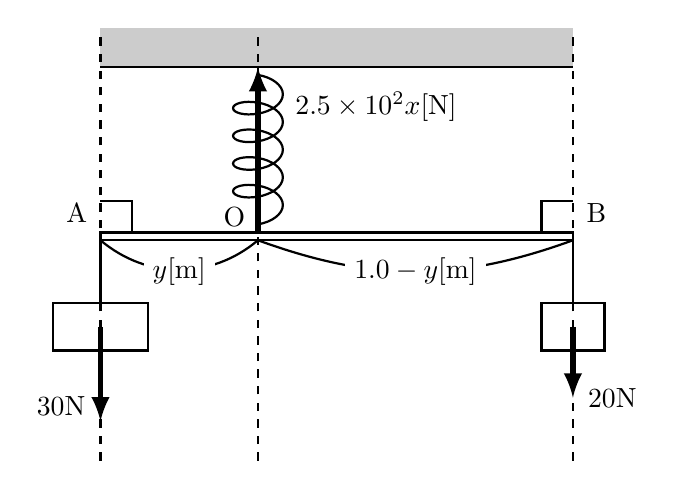
\begin{tikzpicture}[thick]

    \fill[black! 20](0,2) rectangle(6,2.5);
    \draw (0,2)--(6,2);

    \draw (2,2)--(2,1.9);
    \draw[decorate,decoration={coil,amplitude=9pt}] (2,1.9) -- (2,-0.1);

    \draw (0,-0.2) rectangle(6,-0.1);
    \draw (1.7,-0.15) node[above]{O};
    \draw (-0.3,-0.1) node[above]{A};
    \draw (6.3,-0.1) node[above]{B};

    \draw (-0.6,-1.6) rectangle(0.6,-1);
    \draw (0,-0.2)--(0,-1);

    \draw (5.6,-1.6) rectangle(6.4,-1);
    \draw (6,-0.2)--(6,-1);

    \draw[dashed] (0,-3)--(0,2.4);
    \draw[dashed] (2,-3)--(2,2.4);
    \draw[dashed] (6,-3)--(6,2.4);

    \draw (0,0.3)--(0.4,0.3)--(0.4,-0.1);
    \draw (6,0.3)--(5.6,0.3)--(5.6,-0.1);

    \draw[-latex,line width=2pt](0,-1.3)--(0,-2.5);
    \draw (-0.5,-2.3) node{30N};

    \draw[-latex,line width=2pt](2,-0.1)--(2,2);
    \draw (3.5,1.5) node{$2.5\times10^{2}x$[N]};

    \draw[-latex,line width=2pt](6,-1.3)--(6,-2.2);
    \draw (6.5,-2.2) node{20N};

    \draw (0,-0.2)to[out=-40,in=220](2,-0.2);
    \draw (1,-0.6) node[fill=white] {$y$[m]};

    \draw (2,-0.2)to[out=-20,in=200](6,-0.2);
    \draw (4,-0.6) node[fill=white] {$1.0-y$[m]};
  \end{tikzpicture}
\end{figure}


\end{document}